\documentclass[a4paper,12pt]{article}

% Packages
\usepackage{float}
\usepackage[utf8]{inputenc}
\usepackage{fancyhdr}
\usepackage[left = 0.6 in, right = 0.6 in, top = 1 in, bottom = 1 in, headsep = 0.5 in]{geometry}
\usepackage[normalem]{ulem}
\usepackage{enumerate}
\usepackage{pgfplots}
\usepackage{titling}
\pgfplotsset{width=8cm,compat=1.9}
\usepackage{stackengine}
\usepackage{algorithm}
\usepackage[noend]{algpseudocode}
%\pagenumbering{gobble} 
\usepackage{amsmath} % add [fleqn] before {amsmath} to left center
\usepackage{amssymb}
\usepackage[T1]{fontenc}
\usepackage{fancybox}
\usepackage{longtable}

\PassOptionsToPackage{hyphens}{url}\usepackage{hyperref}


\hfuzz = 100pt

%%% Horizontal Line Command
\makeatletter
  \newcommand*\variableheghtrulefill[1][.4\p@]{%
    \leavevmode
    \leaders \hrule \@height #1\relax \hfill
    \null
  }
\makeatother
%%%

%%% Algorithm commands
\algblock{Input}{EndInput}
\algnotext{EndInput}
\algblock{Output}{EndOutput}
\algnotext{EndOutput}
\newcommand{\Desc}[2]{\State \makebox[3em][l]{#1}#2}
%%%

%%% Base conversions
% expandable loop (used to avoid scope problems in tabular cells with the
% standard \loop)
\def\boucle #1\repeat {#1\b@@cle {#1}\repeat \repeat }
\def\b@@cle #1{\repeat #1\b@@cle {#1}}

\makeatletter
\newcount\@nn
\newcount\@mm
\newcount\@base
\newcount\@baseminusone

% please do not use this at home
% #1 must be a counter name, not something expanding to a number.
\def\@arabalpha #1{\ifcase #10\or1\or2\or3\or4\or5\or6\or7\or8\or9\or 
A\or B\or C\or D\or E\or F\or G\or H\or I\or J\or K\or L\or M\or N\or O\or
P\or Q\or R\or S\or T\or U\or V\or W\or X\or Y\or Z\fi}

\newcommand{\baseexpansion}[2][2]{% no negative numbers please!
\def\@digits{}%
\@base#1\relax \@baseminusone\@base\advance\@baseminusone-1
\@nn #2\relax  % this is the number to be written in base #1
%
\ifnum\@baseminusone<36
\def\onerow{#1\kern.1em\hbox{\vrule
   \vtop {\hbox{\ \the\@nn}\kern.3ex\hrule height.1ex }} &%
   \global\@mm\@nn \global\divide\@mm\@base 
   \multiply\@mm\@base \advance\@nn-\@mm 
   \the\@nn \xdef\@digits{\@arabalpha\@nn\@digits}}%
\else
\def\onerow{#1\kern.1em\hbox{\vrule
   \vtop {\hbox{\ \the\@nn}\kern.3ex\hrule height.1ex }} &%
   \global\@mm\@nn \global\divide\@mm\@base 
   \multiply\@mm\@base \advance\@nn-\@mm 
   \the\@nn \xdef\@digits{\the\@nn.\@digits}}%
\fi
%
\leavevmode\oalign{$#2_{10}:$\hfil\cr
      $\left.
      \begin{tabular}{r|l}
         \boucle \onerow \\ \ifnum\@nn>\@baseminusone\global\@nn\@mm \repeat
      \end{tabular}\right\rbrace=
      \mathtt{\@digits}_{#1}$}}     % \hfil removed from the macro

\makeatother

%%% Logic Circuits
\usetikzlibrary{arrows, shapes.gates.logic.US, calc}
\tikzstyle{branch}=[fill, shape=circle, minimum size=3pt, inner sep=0pt]

%%% Header & Footer
\fancyhf{}
\renewcommand{\footrulewidth}{0.1mm}
\fancyhead[L]{Matteo Esposito}
% \fancyhead[R]{COMP 228-AA}
\fancyfoot[R]{\thepage}
\pagestyle{fancy}

%%% Code formatting
\def\code#1{\texttt{#1}}
\renewcommand\maketitlehooka{\null\mbox{}\vfill}
\renewcommand\maketitlehookd{\vfill\null}
\setlength{\abovedisplayskip}{2pt}
\setlength{\belowdisplayskip}{3pt}

%%% Custom settings
% \setlength{\parskip}{1em}  % Paragraph spacing
\setcounter{section}{-1} % Page numbers to start on page 1
\setlength\parindent{0pt} % Remove indenting from entire file
\def\layersep{2.5cm}

%%% Titlepage
\title{\textbf{Data Challenge 1 - ArXiv Article Classification}}
\author{Fundamentals of Machine Learning}
\date{Matteo Esposito (20173298)}

%--------------------------------------------------------------------------%

\begin{document}

\begin{titlingpage}
  \maketitle
  \centering
  \vfill
  {\large{University of Montreal}}\par
  {\large{}}
\end{titlingpage}

\newpage

\section{Introduction}

This report will cover the efforts related to the classification of articles on the popular scientific research paper distribution website, \code{arxiv.org}. 

\medskip

More specifically, given the abstract of several thousand papers, our goal was to classify them into one of the following categories: astro-ph.GA, math.AP, astro-ph.CO, math.CO, stat.ML, cs.LG, gr-qc, astro-ph, astro-ph.SR, hep-th, physics.optics, hep-ph, cond-mat.mtrl-sci, cond-mat.mes-hall, quant-ph.

\medskip

Four types of classifiers were used for the submissions. A random classifier which would randomly assign a class label to each observation with average accuracy of around 6.6\%, followed by a bernoulli and multinomial naive bayes classifier which had average prediction accuracies of 77\% and 79\% respectively and a support vector machine classifier with an average accuracy of 74\%.

\section{Feature Design}

Since at the lowest level we were interested in the count of unique words in our training set abstracts, our feature design could be seen as a dataset condensing/cleaning exercise. All efforts to tidy the dataset were done to reduce the number of unique words/strings (grouping of string characters between spaces) down from over 65,000 to 21,253 which sped up computation times significantly. 

\medskip

\underline{Note:} All cleaning functions were implemented using the following syntax (adapted from the TA's OH notebook): 

\begin{verbatim}
    df[t] = df[t].apply(lambda x : re.sub("<regex pattern>", " ", x))
\end{verbatim}

More specifically, the following changes were done:

\begin{enumerate}
    \item Remove newline characters
    \item Remove punctuation
    \item Remove dollar signs and any mathematical symbols (very important given that many abstracts had mathematical terms and functions)
    \item Remove standalone integers 
    \item Make all strings lowercase
    \item Strip all strings of spaces (using x.strip())
    \item Remove all common stopwords
\end{enumerate}

\section{Algorithms}

The algorithms considered and implemented in this kaggle were the following:
\begin{enumerate}
    \item \textbf{Random Classifier}. Randomly assign class labels from the training set to the test set observations.
    \item \textbf{Bernoulli Naive Bayes Classifier} using base python and numpy. Binarize data (1 if the word is in the given abstract, otherwise 0) for all unique words in vocabulary. Calculate prior and likelihoods/conditional probabilities to get class probabilities (posteriors). Assign class associated with max posterior probability as predicted class.
    \item \textbf{Multinomial Naive Bayes Classifier} from the sklearn library including the use of CountVectorizer, TfidfTransformer and Pipeline. Same as above, however, we are interested in the actual number of times a given word appears in an abstract.
    \item \textbf{Support Vector Machine Classifier} from the sklearn library including the use of CountVectorizer, TfidfTransformer and Pipeline.
\end{enumerate}

\section{Methodology}

For all experiments, a train/validation split of 70/30 was used. When it came time to submit a final submission, I trained the models on the entire training set (i.e. a split of 100/0) in an effort to maximize the generalizability of the model being used. 

\medskip

The distribution choice for the NB classifier was predetermined to be Bernoulli. 

\medskip

There was no regularization strategy (aside from a naive grid search in the SVM implementation), however, to optimize the hyperparameters (namely alpha in the case of the NB classifiers), a grid search was implemented. The results of these grid searches can be seen in the results section of this report.

\section{Results}

As detailed in Figure 1, the results for the random classifier were very poor. The average prediction accuracy of roughly 6.6\% is reasonable in our application since we are randomly assigning 1 of 15 labels with equal weight. $\frac{1}{15} = 0.066 = 6.6\%$. The kaggle result for this submission was 0.06755, not beating the random baseline.

\begin{figure}[H]
    \centering
    \caption{Random Classifier Accuracy Comparison}
    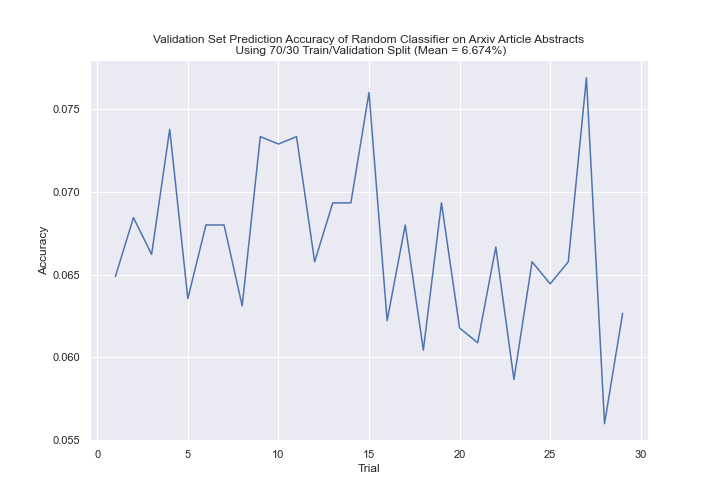
\includegraphics[width=12cm]{compareRandom.png}    
\end{figure}

Performing a gridsearch on alpha values among [0.01, 0.05, 0.1, 0.15, 0.3, 0.5, 1], we observed that the optimal value for Bernoulli NB was 0.3 and 0.15 for Multinomial NB. They yielded the prediction accuracies below:

\begin{table}[H]
    \centering
    \caption{Table of Naive Bayes Prediction Accuracies}
    \begin{tabular}{|c|c|c|c|c|}
        \hline
        \text{\textbf{Model}} & $\alpha$ & \text{\textbf{In Development}} & \text{\textbf{Public Leaderboard}} & \text{\textbf{Private Leaderboard}} \\ \hline
        Bernoulli NB & 0.3 & 0.774 & 0.778 & 0.781 \\ \hline
        Multinomial NB & 0.15 & 0.793 & 0.801 & 0.794 \\ \hline
    \end{tabular}
\end{table}

The Bernoulli and Multinomial scores beat the Numpy only and best baselines respectively.

\begin{figure}[H]
    \centering
    \caption{Bernoulli NB and Multinomial NB Accuracy Comparison}
    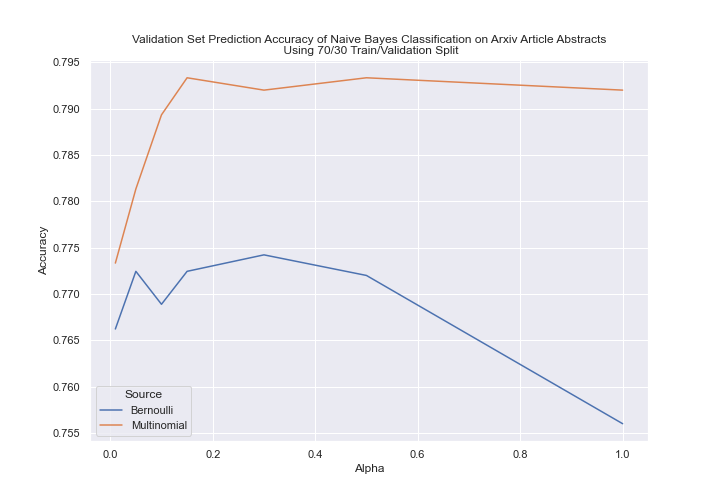
\includegraphics[width=12cm]{compare.png}    
\end{figure}

The final and second of the experimental algorithms implemented was a linear support vertor machine using stochastic gradient descent by means of the SGDClassifier module of the sklearn.linear model package. Here we used hinge loss, l2 regularization and preformed a grid search of alpha (regularization multiplier) terms among $[0.001, 0.005, 0.0075, 0.01, 0.02]$ and a grid search among max iteration/epoch values of $[5, 10, 20, 50]$. The optimal parameters yielded an average prediction accuracy of around 74\%.

\medskip

This model pipeline had the exact same preprocessing steps as in the multinomial nb implementation, namely the use of the cleaned data from the bernoulli nb implementation and the use of CountVectorizer and TfidfTransformer.

\begin{figure}[H]
    \centering
    \caption{SVM Grid Search Results}
    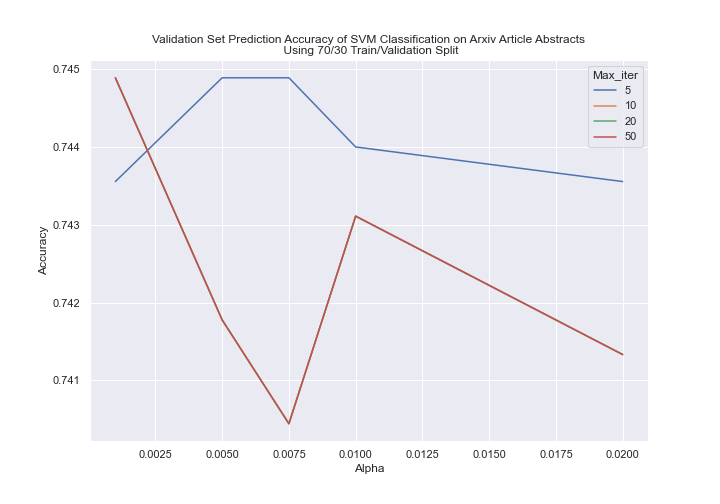
\includegraphics[width=12cm]{compareSVM.png}    
\end{figure}

\section{Discussion}

As a general observation, we could have used ensembling techniques to improve the accuracy of the model as none were actually used in all the work that was done in this data challenge.

\medskip

Known pros of the \textbf{Naive Bayes classification} include the fact that it is good with independent data and is particularly well suited to tasks such as text classification. The downsides of NB come at runtime where applying smoothing is an additional step in the conditional probability/likelihood calculation step which adds to the runtime. Sparsity and very small probabilities are also an issue in NB, to which we present a potential solution below.

\medskip

An area that could have significantly improved model performance here would be word stemming. This is the process by which we reduce inflected or derived words to their base or root form (source: \url{https://en.wikipedia.org/wiki/Stemming}). This would have a 2 fold effect. It would reduce the size of our dictionary which even after all of the data cleaning steps performed, was still over 21,000 words long. In consequence, it would increase the training and predicting speed to allow for more testing and experiements.

\medskip

Concerning \textbf{SVMs}, a pro would be that it is particularly well suited for high dimensional data, which is very much the situation that we are in. 15000 observations and over 21000 features in our testing set can be considered high dimensional. SVM is good for high dimensional data since, unlike other algorithms, it doesn't need to evaluate every single point in the data set to draw its decision boundary. It observes a subset that will build its support vectors so that it can set the best decision boundary.

\medskip

On the other hand, a con would be that there were a large choice of hyperparameters to modulate and optimize. A very small amount of time was invested into optimizing these since at this point, I had already beaten the best baseline with my multinomial NB implementation. In particular, modulating the choice of kernel would likely yield a better decision boundary and therefore, a better ability to generalize.

\medskip

For the SVM implementation, since the maximum number of iterations hyperparameter did not have any postive effect on the prediction accuracy when at a value of 10 or greater, perhaps an improvement could be seen with maximum number of iterations values less than 10. The only value lower than 10 tested was 5 which yielded up to a 0.5\% improvement in predictions. The reasonable alpha parameters seem to be between 0 and 0.01 and therefore the range of alpha values selected for the grid search can remain and are appropriate.

\section{References}

\begin{enumerate}
    \item Multinomial NB documentation: \url{https://scikit-learn.org/stable/modules/generated/sklearn.naive_bayes.MultinomialNB.html} and \url{https://medium.com/@anuuz.soni/pros-and-cons-of-naive-bayes-classifier-40b67249ae8}
    \item SGD Classifier documentation: \url{https://scikit-learn.org/stable/modules/generated/sklearn.linear_model.SGDClassifier.html}
    \item Multinomial NB Implementation: \url{https://towardsdatascience.com/multinomial-naive-bayes-classifier-for-text-analysis-python-8dd6825ece67}
    \item NLP Implementation: \url{https://towardsdatascience.com/machine-learning-nlp-text-classification-using-scikit-learn-python-and-nltk-c52b92a7c73a}
\end{enumerate}


% \textbf{a)} Since $2^6 = 64$ and $2^7 = 128$, if we are dealing with 87 unique instructions it is clear that we need 7 out of the 24 available bits from the standard word size to represent our instruction/opcode set.

% \textbf{b)} Since we have 17 remaining bits for memory addresses, the maximum value that can be represented in binary is $2^{18}-1 = 262143_{10}$.

% \textbf{c)} Knowing that the range of N-bit 2s complement values is $[-2^{n-1}, 2^{n-1}-1]$, and considering that we have 24 bit words, the range and max of 2s complement values is: 

% $$[-2^{n-1}, 2^{n-1}-1] = [-2^{23}, 2^{23}-1] = [-8388608, 8388607] \Rightarrow \fbox{8388607}$$

% \subsection*{Question 2}

% Interpreting each set of 4 bits from the Marie snippet \code{121830F46000900A}, where bit 1 represents the instruction number and bits 2-4 the memory address, we get the 4 following instructions:

% \begin{table}[H]
%     \centering
%     \begin{tabular}{|c|c|c|c|}
%         \hline
%         \text{\textbf{Hex}} & \text{\textbf{Opcode}} & \text{\textbf{Address}} & \text{\textbf{Instruction}} \\ \hline
%         1218 & 1 = \code{LOAD} & $218_{16}$ & \code{LOAD 218} \\ \hline
%         30F4 & 3 = \code{ADD} & $0F4_{16}$ & \code{ADD 0F4} \\ \hline
%         6000 & 6 = \code{OUTPUT} & - & \code{OUTPUT} \\ \hline
%         900A & 9 = \code{JUMP} & $00A_{16}$ & \code{JUMP 00A} \\ \hline
%     \end{tabular}
% \end{table}

% \subsection*{Question 3}

% % \begin{figure}[H]
% %     \centering
% %     \caption{Timing digram for \code{LOADI} instruction}
% %     \includegraphics[width=12cm]{figures/q3.jpg}    
% % \end{figure}

% \subsection*{Question 4}

% \textbf{a)} Converting every bit in $AAFB1609_{16}$ to binary, we get,

% $$AAFB1609_{16} = 10101010111110110001011000001001_{2}$$

% Converting this to two's complement notation (flip all bits and add 1) we get,

% $$10101010111110110001011000001001_{2} \rightarrow 
% -(01010101000001001110100111110110_{2})$$

% then,

% $$-(01010101000001001110100111110110_{2}) + 1 =
% -(01010101000001001110100111110111_{2})$$

% converting back to decimal,

% $$-(01010101000001001110100111110111_{2}) = -1426385399$$

% \textbf{b)} Converting every bit in $0916FBAA_{16}$ to binary, we get,

% $$0916FBAA_{16} = 00001001000101101111101110101010_{2}$$

% Using the IEEE standard for single precision floating point numbers, namely to use bit 1 as the sign bit, the next 8 for the exponent and remaining 23 for the mantissa we get,

% $$0|00010010|00101101111101110101010$$

% This yields an exponent value of $00010010_2 = 18_{10}$. If we inversely apply the bias to get the original value of the exponent, we have 18 - 127 = -109. If we convert the mantissa, we get $1.00101101111101110101010_{2} \; x \; 2^{-109}$. We will translate the solution by 1 power to the right. $0.1001 0110 1111 1011 1010 1010_{2} \; x \; 2^{-108}$. Converting to hex then decimal we get the following:

% \begin{align*}
%     0.96FBAA_{16} \; x \; 2^{-108} &= (9\cdot16^{-1} + 6\cdot16^{-2} + 15\cdot16^{-3} + 11\cdot16^{-4} + 10\cdot16^{-5} + 10\cdot16^{-6}) \; x \; 2^{-108} \\
%     &= 0.589777589 \; x \; 2^{-108}        
% \end{align*}

% Converting $2^{-108}$ to an exponent of 10, we get:

% \begin{align*}
%     2^{-108} &= 10^{x} \\
%     -108 \cdot log_2(2) &= x\cdot log_2(10) \\
%     \frac{-108}{log_2(10)} &= x \\
%     -32.5112395 &\approx x
% \end{align*}

% finally,

% $$0.589777589 \; x \; 2^{-108} = 0.589777589 \; x \; 10^{-32.5112395}$$

% To get a whole number exponent, we can multiply the coefficient by a constant.

% $$\frac{0.589777589}{10^{-33+32.5112395}} \; x \; (10^{-32.5112395})*(10^{-33+32.5112395}) = 1.8173926 \; x \; 10^{-33}$$

% \subsection*{Question 5}

% $$Q = (A+B)/C - D*E$$

% \textbf{a)} 

% \begin{align*}
%     &\code{Push A} \\
%     &\code{Push B} \\
%     &\code{add} \\
%     &\code{Push C} \\
%     &\code{Div} \\
%     &\code{Push D} \\
%     &\code{Push E} \\
%     &\code{Mult} \\
%     &\code{Sub} \\
% \end{align*}

% Following the \code{Sub} call, we need to store/pop the final result (Q) from the stack.

% \textbf{b)}

% \begin{align*}
%     &\code{Add R1, A, B} \\
%     &\code{Div R2, R1, C} \\
%     &\code{Mult R3, D, E} \\
%     &\code{Sub R4, R2, R3} \\
% \end{align*}

% Q will be stored in register R4.

% \subsection*{Question 6}

% Calling \code{LOAD 500}.

% \begin{figure}[H]
%     \centering
%     \begin{tabular}{|c|c|}
%         \hline
%         \textbf{Mode} & \textbf{Value Loaded into AC}  \\ \hline
%         \text{Indirect} & 100\\ \hline
%         \text{Indexed} & 300\\ \hline
%         \text{Direct} & 300\\ \hline
%         \text{Immediate} & 500\\ \hline
%     \end{tabular}
% \end{figure}

% \subsection*{Question 7}

% See \code{mult.mas}.
% \par
% \underline{Note:} All inputs must be entered in the ASCII (default) input setting for correctly formatted output.

\end{document}